\documentclass[main]{subfiles}

\begin{document}


\chapter{Simulaciones del modelo f\'isico}
\label{chap:simulador}

Luego de desarrollado un modelo f\'isico resulta fundamental disponer de un entorno para realizar simulaciones. Las razones para construir un simulador son evidentes. En primer lugar resulta fundamental para comprobar que el modelo realizado se comporta acorde a lo que uno espera a priori del sistema. Para este tipo de pruebas se trabajar\'a con las situaciones m\'as sencillas en las cuales se puede calcular la trayectoria trivialmente. El segundo objetivo del simulador es poder conocer el comportamiento de nuestro sistema frente a algunas acciones de control determinadas. Por ejemplo conocer la trayectoria que desarrolla el cuadric\'optero si accionamos solamente uno de los motores o cualquier combinaci\'on que sea pertinente de estudio. El simulador es utilizado tambi\'en para verificar el funcionamiento del Filtro de Kalman Extendido realizado para la integraci\'on de los sensores (Ver capo \'tulo \ref{kalman}). Se puede generar una trayectoria a la cual se le agrega ruido que simule el ruido de medida de los sensores. Luego se puede comparar la trayectoria obtenida con el filtrado de Kalman con la generada inicialmente. Por 	ltimo y fundamentalmente el simulador ser\'a clave para testear y mejorar los algoritmos de control desarrollados. Previo a testear con el sistema real y a fin de evitar da\~nos sobre el mismo, se deben verificar dichos algoritmos en el simulador. Por los motivos expresados es necesario que el simulador represente fielmente el modelo f\'isico y se comporte acorde a la realidad. \\

El dise\~no del simulador se realiza utilizando Simulink. Dado que se debe trabajar con funciones que no dependen exclusivamente del tiempo, no fue posible desarrollar un simulador que resolviera directamente las ecuaciones diferenciales que gobiernan al sistema utilizando un m\'etodo m\'as directo, como por ejemplo \emph{ODE45}. 



\section{Estructura del Simulador}

El simulador se compone de tres elementos fundamentales. El lazo abierto, es decir las ecuaciones que gobiernan al cuadric\'optero. En dicho sistema tenemos como entradas las velocidades angulares del sistema sobre las cuales realizaremos las acciones de control y como salidas tenemos el vector de estados del sistema en todos los instantes desde el tiempo inicial establecido en la simulaci\'on hasta el tiempo final. Se compone adem\'as de un bloque encargado de generar las rutas a seguir por el cuadric\'optero a partir de los \emph{waypoints} que se ingresen. Finalmente una tercer parte que se encarga de simular el control. Este \'ultimo bloque se vale de los dos anteriores.

\subsection{Lazo Abierto}

La estructura que se eligi\'o para desarrollar esta secci\'on se corresponde en buena forma con el camino que se recorri\'o para determinar el modelo. Por dicho motivo la estructura de esta parte del simulador se descompone en tres bloques. En la figura \ref{fig:lazo_abierto} se observa la estructura global del lazo abierto. En la figura \ref{fig:vista} se observa una captura de pantalla que representa la vista general de la parte encargada de simular el lazo abierto.
\begin{figure}[h!]
	\centering
	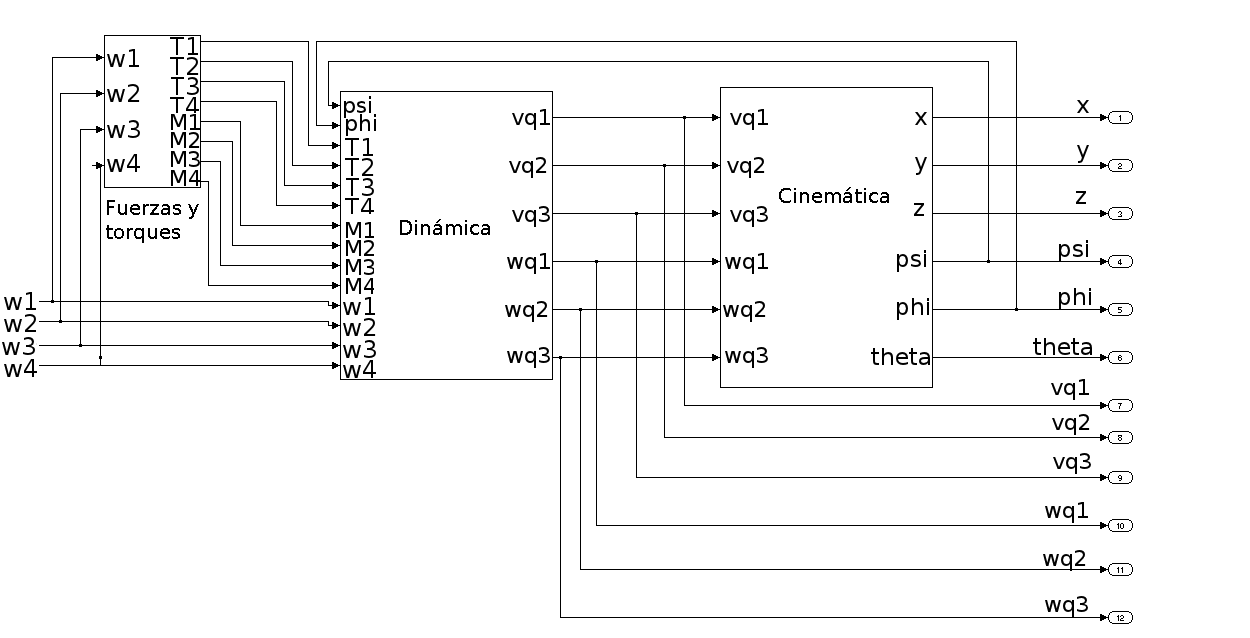
\includegraphics[width=1\textwidth]{./pics_simulador/lazo_abierto.png}
	\caption{Bloque de lazo abierto}
	\label{fig:lazo_abierto}
\end{figure}

\begin{figure}[h!]
	\centering
	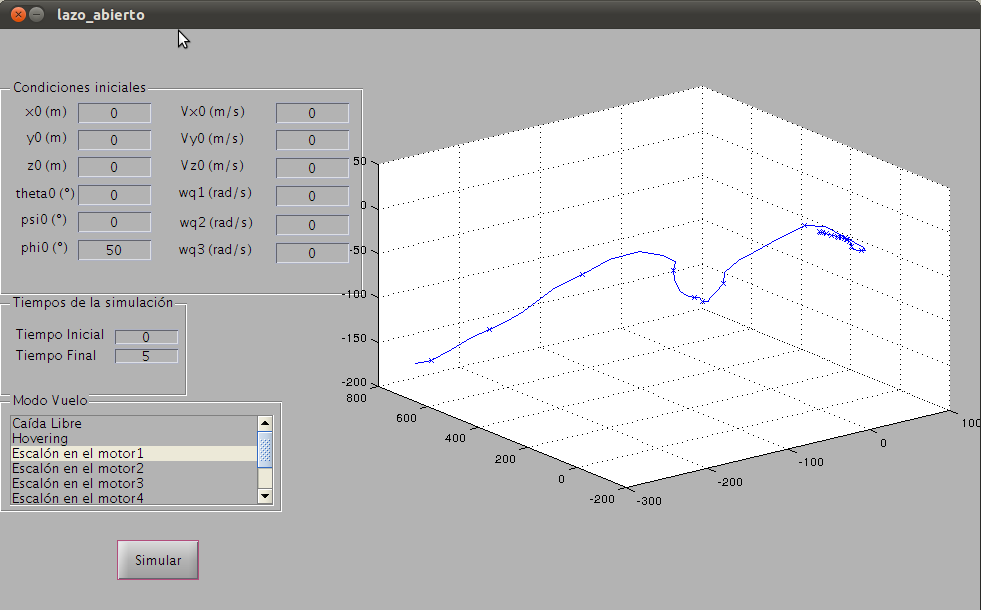
\includegraphics[width=1\textwidth]{./pics_simulador/vista.png}
	\caption{Interfaz del simulador de lazo abierto}
	\label{fig:vista}
\end{figure}
\subsubsection{Cinem\'atica}

En la figura \ref{fig:cinematica} se puede observar un diagrama de bloques de la parte del sistema que transforma las velocidades lineales y angulares en posiciones y ángulos de Euler. Se distinguen dos sub-bloques principales, uno encargado de devolver la  posici\'on y otro encargado de devolver los \'angulos de Euler
\begin{figure} [h!]
  \centering
  \subfloat[Bloque cinem\'atica]{\label{fig:cinematica}
  		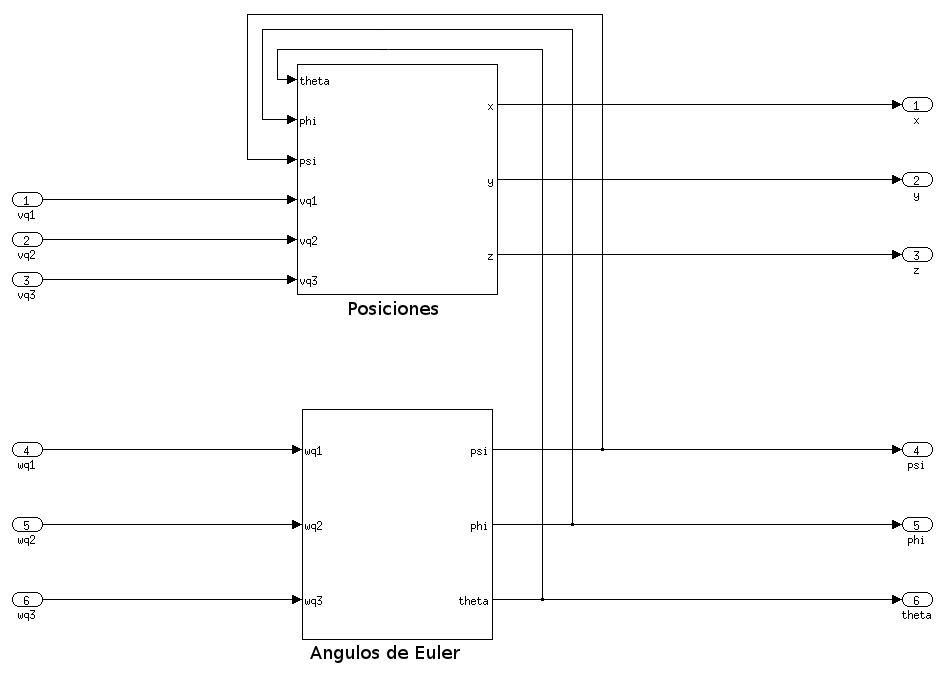
\includegraphics[width=0.6\textwidth]
  			{./pics_simulador/cinematica.png}}
  \subfloat[Bloque din\'amica]{\label{fig:dinamica}
  		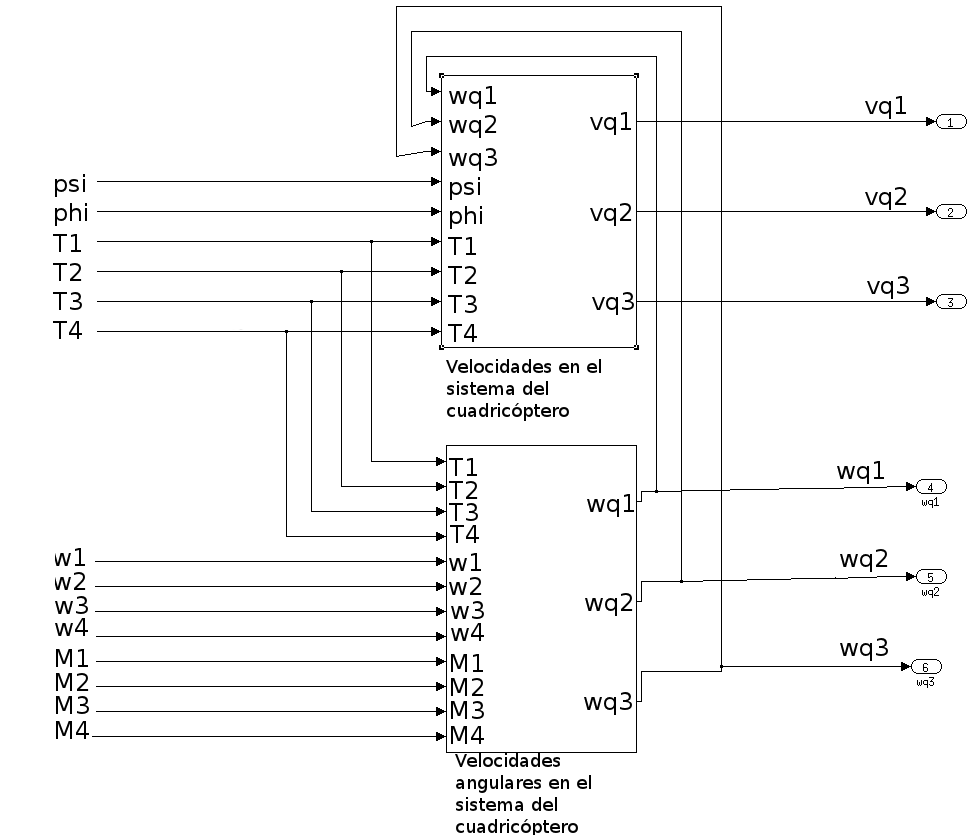
\includegraphics[width=0.5\textwidth]
  			{./pics_simulador/dinamica.png}}
  \caption{Bloques en mayor detalle}
  \label{fig:bloques}
\end{figure}



\subsubsection{Din\'amica}

Al igual que el bloque anterior, se divide este en dos sub-bloques m\'as (ver figura \ref{fig:dinamica}). Los bloques en este caso son el que devuelve las velocidades angulares y las lineales. 


\section{Simulaciones}
En esta secci\'on procedermos a realizar algunas simulaciones a fin de verificar que los resultados arrojados se corresponden con lo esperado a priori. 

\subsubsection{Ca\'ida libre con velocidad inicial nula}

Se simula una ca\'ida libre con condiciones iniciales nulas excepto la altura que se fija a $100m$. El tiempo de simulaci\'on considerado es de tres segundos. En la figura \ref{fig:clv0} se observa la trayectoria obtenida. En este caso se graf\'ica uno de cada cinco puntos obtenidos. La misma se corresponde con lo que se espera a priori. En la figura \ref{fig:zcl} se representa la altura en funci\'on del tiempo. La altura final es $z_f=55.855$. La altura en una caida libre puede calcularse como $z(t)=-\frac{gt^2}{2}+Z_0$. En este caso se obtiene $z(3)=55.855$.



\begin{figure} [h!]
  \centering
  \subfloat[Trayectoria de caida libre con velocidad inicial nula]{\label{fig:clv0}
  		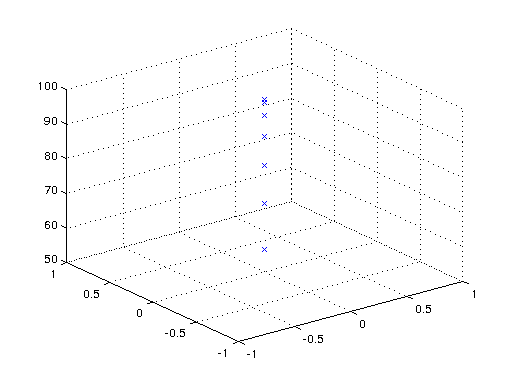
\includegraphics[width=0.5\textwidth]
  			{./pics_simulador/clv0.png}}
  \subfloat[Altura en funci\'on del tiempo]{\label{fig:zcl} 
  		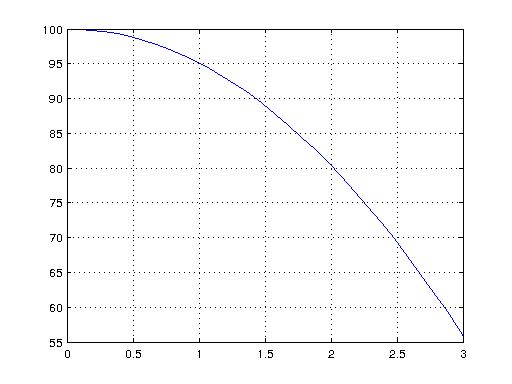
\includegraphics[width=0.5\textwidth]
  			{./pics_simulador/clz.png}}
 
  \caption{Caida libre con velocidad inicial nula}
  \label{fig:caida_libre}
\end{figure}

\subsubsection{Ca\'ida libre con velocidad inicial}
Se realiza la misma simulaci\'on que en la secci\'on anterior excepto que se inicia el vuelo con $V_0 = 1ms^{-1}\vec{i}+3ms^{-1}\vec{k}$. Tal como es de esperar en la posici\'on seg\'un $\vec{i}$ se tiene una posici\'on que aumenta con el tiempo con pendiente igual a la velocidad inicial. La altura cumple que $z(t)=-\frac{gt^2}{2}+3ms^{-1}t+Z_0$. Por lo tanto la misma aumenta hasta un tiempo  $t^* / \dot{z(t)=0}$. Lo cual implica que $t*=\frac{3ms^{-1}}{g}\approx0.31s$. Por otra parte tiempo para el cual se da el m\'aximo en la simulaci\'on es $t_{max} \approx 0.33s$. Considerando que las simulaciones se realizan con un paso variable el cual puede ser de hasta $0.1s$ se considera un resultado aceptable. Por otra parte la altura m\'axima en teor\'ia vale $z_{max_{teo}}=100.459m$ mientras que la altura m\'axima obtenida a trav\'es de la simulaci\'on es de $z_{max_{sim}}=100.456m$. Esta diferencia puede explicarse gracias a que estamos evaluando la trayectoria en tiempos distintos. A partir de este punto tenemos una ca\'ida libre como la que ya estudiamos en el caso anterior. Las alturas finales, tanto en la simulaci\'on como en la teor\'ia valen $64.885m$.

\begin{figure} 
  \centering
  \subfloat[Trayectoria de caida libre con velocidad $V_0 = 1ms^{-1}\vec{i}+3ms^{-1}\vec{k}$]{\label{fig:clv1}
  		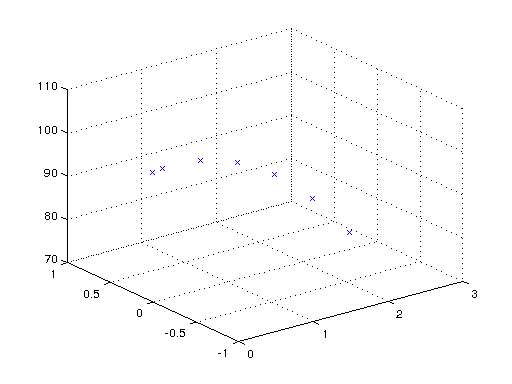
\includegraphics[width=0.35\textwidth]
  			{./pics_simulador/clv1.png}}
  \subfloat[Altura en funci\'on del tiempo]{\label{fig:clzv1} 
  		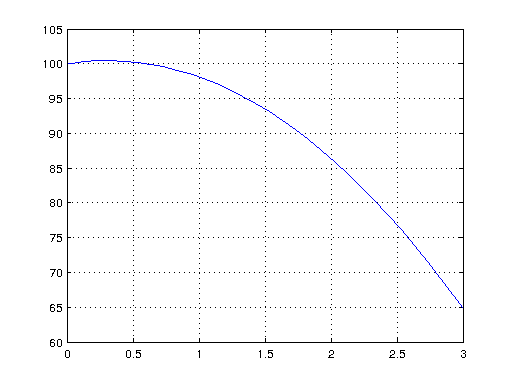
\includegraphics[width=0.35\textwidth]
  			{./pics_simulador/clzv1.png}}
   \subfloat[Desplazamiento hacia el Este en funci\'on del tiempo]{\label{fig:clxv1} 
  		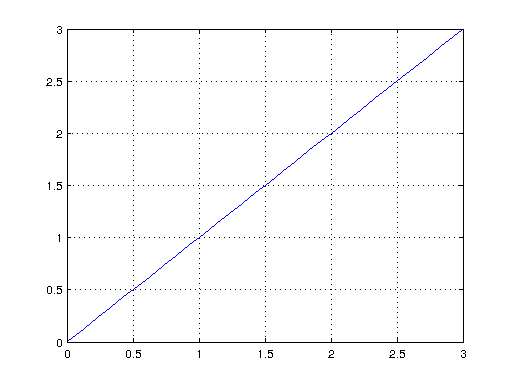
\includegraphics[width=0.35\textwidth]
  			{./pics_simulador/clx1.png}}   			
 
  \caption{Caida libre con velocidad inicial no nula}
  \label{fig:caida_libre_vi}
\end{figure}


\subsubsection{Condici\'on de Hovering}

Se aplica una fuerza constante en los cuatro motores tal que la resultante es igual al peso. Las condiciones iniciales son todas nulas. Excepto $Z_0=10m$. Se logra el equilibrio mec\'anico. Todas las variables permanecen constantes. Se simula durante diez segundos

\subsubsection{Giro seg\'un el eje $\vec{k}$}

En las mismas condiciones que la simulaci\'on anterior, se aumenta repentinamente la velocidad angular de los motores que rotan en sentido horario con un valor tal que la fuerza de cada uno de esos motores aumenta en $1N$. Para los motores que rotan en sentido anti-horario se disminuye la velocidad angular de forma que la fuerza de cada uno de ellos disminuye $1N$. Estas velocidades son $375.03rads^{-1}$ y $287.68rad^{-1}$ La fuerza neta y el momento seg\'un los versores $\vec{i_q}$ y $\vec{j_q} $ es nulo. Sin embargo aparece un torque negativo seg\'un el versor $\vec{k_q}$.\\

En la figura \ref{fig:hovz} se presenta la altura en funci\'on del tiempo. La misma deber\'ia permanecer constante sin embargo se observa una peque\~na diferencia en la altura de $3cm$. Esta diferencia es atribuida a un error num\'erico a la hora de calcular las velocidades con las cuales deben girar los motores. Por otra parte en la figura \ref{fig:hovtheta} se observa como el \'angulo decrece hasta el valor de $-108.77 rad$. El torque neto vale $Q = -0.38Nm $. Por lo tanto en 5 segundos se debe rotar un \'angulo de $\theta_f=-108.42$. Nuevamente se percibe una peque\~na diferencia entre el valor te\'orico y el simulado. Sin embargo dicho error es completamente aceptable. 



\begin{figure} [h!]
  \centering
  \subfloat[Altura en funci\'on del tiempo]{\label{fig:hovz}
  		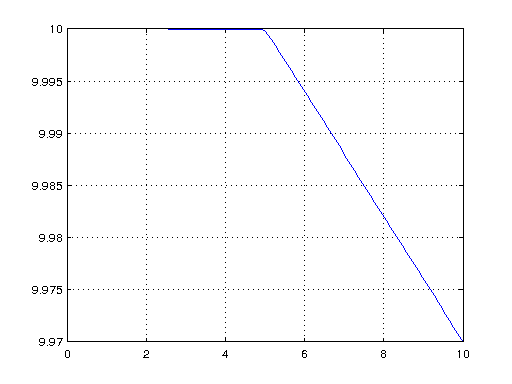
\includegraphics[width=0.5\textwidth]
  			{./pics_simulador/hovz.png}}
   \subfloat[\'Angulo de Yaw]{\label{fig:hovtheta} 
  	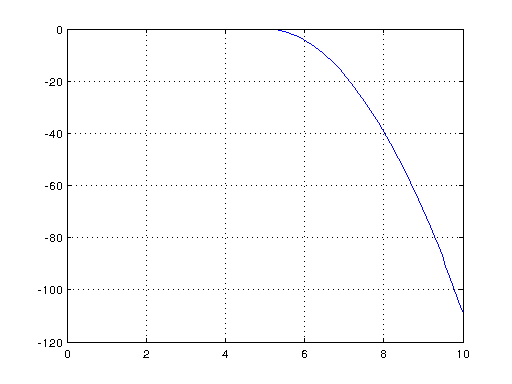
\includegraphics[width=0.5\textwidth]
  			{./pics_simulador/hov_theta.png}} 
  \caption{Giro seg\'un el $\vec{k_q}$}
  \label{fig:hov}
\end{figure}

\subsubsection*{Vuelo en linea recta}

Con condiciones inicial nulas, excepto por $Z_0 = 10m$ y $\varphi = 30 ^{\circ}$. Se simula durante diez segundos. En la figura \ref{fig:recta} se observa un vuelo en linea recta en la direcci\'on $\vec{i}$. Como es de esperar el vuelo ser\'a uniformemente acelerado ya que la fuerza es siempre en el sentido de $\vec{k_q}$. La simulaci\'on arroja que al cabo de diez segundos el desplazamiento es de $283.19m$, mientras que en la teor\'ia se obtiene un desplazamiento de $218.20m$	. Nuevamente se concluye que los resultados arrojados por el simulador son satisfactorios.

\begin{figure}[h!]
	\centering
	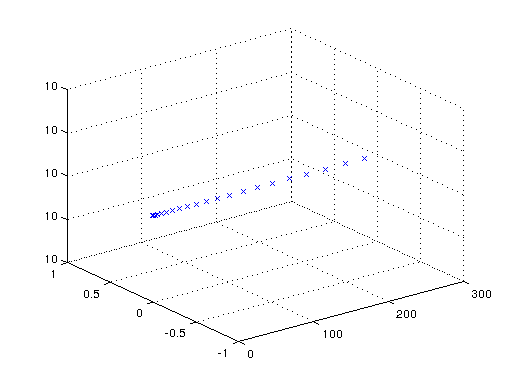
\includegraphics[width=1\textwidth]{./pics_simulador/recta.png}
	\caption{Vuelo en linea recta}
	\label{fig:recta}
\end{figure}

Hasta aqu\'i hemos testeado el simulador en situaciones conocidas. De acuerdo a las pruebas realizadas puede afirmarse que su funcionamiento es el adecuado ya que en ninguna prueba se obtuvieron errores considerables. 

\end{document}